\chapter{Resultat  –  en numerisk beskrivning av energiflöden}

I detta kapitel presenteras de resultat som erhållts med hjälp av metodiken i föregående kapitel. De olika delresultaten visar på olika typer av energiflödens karaktär och hur de påverkas av väderparametrarna. Kapitlet avslutas med sammanställning av de individuella bidragen i from av en free-running temperature.

Genom att beräkna storlekarna av energiflödena genom byggnadens olika delar kan vi se var energiflödena är som störst vid olika väderförhållanden. Vi har valt att titta på en klar dag i mitten av april då solinstrålningen når en topp vid $\unit[640]{W/m^2}$ och solen är uppe i 14 timmar. Dygnets temperatur varierar mellan $\unit[6]{^\circ C}$ och $\unit[9]{^\circ C}$ och vinden är runt $\unit[10]{m/s}$. Enligt väderstatistik från SMHI\cite{SMHIdata} bör detta vara en rimlig dag med väldigt bra väder vid den valda tiden på året.

Vi vald en dag med fint väder eftersom energiflödena då är små och kan de förbättras när de är små, kan de också förbättras när de är stora. Att vi valde en dag i april beror på att det fortfarande är under eldningssäsongen, det vill säga den tid på året då man fortfarande värmer upp huset. Eldningssäsongen för fastigheten på Walleriusgatan är ungefär från början oktober till slutet av april. Under sommaren sker ingen uppvärmning.


\section{Konstanta energiflöden}

En del av energiflödena är relativt konstanta sett till en längre tidsperiod. Dessa är främst värme från elektriska apparater, så som kylskåp och datorer, människors kroppsvärme och varmvattencirkulation. Även kylningen från husets grund anses vara konstant.

Väldigt liten del av den energi som förbrukas i en elektrisk apparat blir till något annat än värme. Därför låter vi det energiflödet motsvaras av fastighetens energiförbrukning. Den kan läsas av kontinuerligt och på så sätt reglera aktivt tillförd energi\footnote{Aktivt tillförd energi: Den energitillförsel som kan regleras och tillförs via radiatorerna.}.

Människornas utstrålade kroppsvärme kan beräknas genom att de antas vara svartkroppar. Stefan-Boltzmanns lag säger då att utstrålade energi per yt- och tidsenhet är $j=\sigma T^4$, där $T$ är temperaturen och $\sigma=\unit[5.6705\cdot 10^8]{Wm^{-2}K^{-4}}$ \cite{physicshandbook}. På samma sätt beräknas den energi som strålas in mot kroppen från omgivningen. Nettostrålningen från en människa kan då ses i ekvation \eqref{eq:constantsources:stefan} där $T_k=37^{\circ}C=310K$ är kroppstemperaturen och $T_r=20^{\circ}C=293K$ är rumstemperaturen. Multiplicerat med en människas area, ungefär $\unit[2]{m^2}$, fås en nettoeffekt på $\unit[211]{W}$. I själva verket reduceras denna effekt av en rad faktorer. Exempelvis är hudens temperatur lägre än kroppstemperaturen samtidigt som klädesplagg reducerar effektutstrålningen något. Det är allmänt vedertaget att man kan sätta nettoeffekten till ungefär $\unit[50-100]{W}$.

\begin{equation}
\label{eq:constantsources:stefan}
j=\sigma \left( T_k^4 - T_r^4 \right)
\end{equation}
\noindent
I huset cirkulerar hela tiden varmvattnet för att alltid kunna tillgodose de boendes behov av varmvatten utan dröjsmål. Efter en tur i systemet sjunker temperaturen på varmvattenet med tre grader. Detta motsvarar en energitillförsel till fastigheten på \textcolor{red}{??} $\unit[]{W}$.

Grunden huset står på har en randtemperatur på ungefär $6^{\circ}\mbox{C}$ från marken. Den kan antas vara konstant då huset grund ligger en bit ned under marken. Enligt SLU, Sveriges Lantbruksuniversitet, kan marktemperaturen antas vara konstant från $\unit[1,6]{m}$ under markytan \cite{SLU}. Deras data kommer från Uppsala vilket borde vara jämförbart med Göteborg. Huset står på en grund som består av ett luftgap och sedan $\unit[0,25]{m}$ betong. Längst ned i huset finns en källare som är ouppvärmd \textcolor{red}{??}. Det energiläckage som då blir genom husets grund ned i marken kan beräknas uppgå till \textcolor{red}{??} $\unit[]{W}$.


\subsection{Energiflöde genom väggar}

\subsection{Flöde vid termisk jämvikt}
\label{sec:steadystatewall}

%To regerenate the figures use /code/pdesolver/generateWallFigApril.m
%with the argument /code/pdesolver/walldata.mat


För att visualisera flödet genom en vägg vid konstant väder och utomhustemperatur görs 
beräkningar med finita elementmetoden och en konstant inomhustemperatur på 
$\unit[20]{^\circ C}$. Utomhusvädret är relativ konstant och är satt till antingen molning 
eller klart och utomhustemperaturen varierar mellan $\unit[6]{^\circ C}$ på natten och 
$\unit[9]{^\circ C}$ på dagen. Detta har gjorts för en vägg utan och en vägg med 
isolering, se figur \ref{fig:energyflow_stst}. Den oisolerade väggen består av 
$\unit[0,5]{m}$ tegel och den isolerade har dessutom $\unit[0,1]{m}$ mineralull. 

\begin{figure}[hpbt]
\centering

\subfloat[Energiflöde ut från insidan av en oisolerad vägg en klar dag.]{
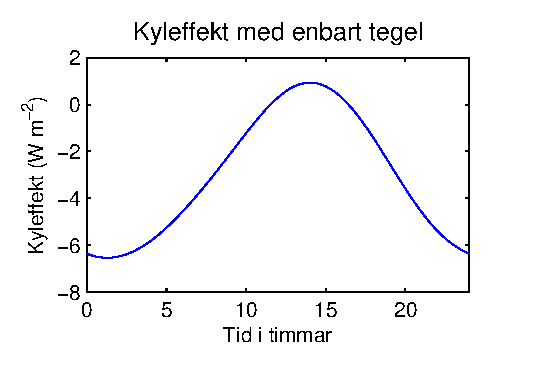
\includegraphics[width=6cm]{images/noinsulationapril.eps}}\vspace{1cm}
\subfloat[Energiflöde ut från insidan av en isolerad vägg en klar dag.]{
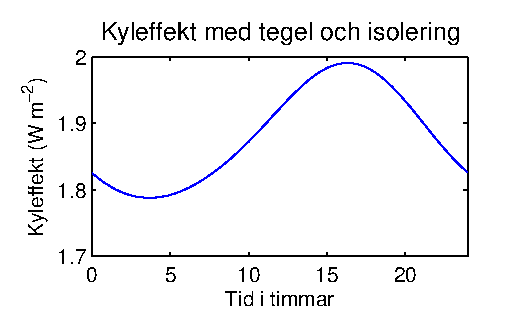
\includegraphics[width=6cm]{images/insulationapril.eps}
}

\subfloat[Energiflöde ut från insidan av en oisoleradvägg en molnig dag.]{
\includegraphics[width=6cm]{images/noinsulationcloud.eps}}\vspace{1cm}
\subfloat[Energiflöde ut från insidan av isolerad vägg en molnig dag.]{
\includegraphics[width=6cm]{images/insulationcloud.eps}
}

\caption{\label{fig:energyflow_stst} Energiflöden ut från insidan av en vägg en dag motsvarande en i mitten av april.
Utomhustemperaturen varierar mellan $\unit[6]{^\circ C}$ på natten och $\unit[9]{^\circ C}$ på dagen. Inomhustemperaturen är satt konstant $\unit[20]{^\circ C}$.}
\end{figure}


%RESULTAT ur graferna 
I figurerna \ref{fig:energyflow_stst} kan vi se att energiflödet genom väggen minskar till 
ungefär en fjärdedel med isolering. Under ett soligt dygn kommer det att flöda värme in i
 fastigheten. På grund av fördröjningen i väggen sker detta främst under natten, 
 och mindre på dagen. Med isolering blir variationen mindre och ett mindre men jämnare 
 energiflöde, under $\unit[1]{W m^{-2}}$, går i fastigheten under hela dygnet.

Under en motsvarande fast molnig dag varierar energiflödet mellan 7 och 10 
$\unit{W m^{-2}}$ till att röra sig mellan 2,1 och 2,3 $\unit{W m^{-2}}$, dock ut ur 
fastigheten. En isolering innebär ett minskat energiutflöde och därmed en minskad 
energiförlust för fastigheten.

Trots att energi flödar in i fastigheten den soliga dygnet så flödar ganska mycket energi 
ut ur fastigheten under det molniga dygnet. Göteborg har 1800 solskenstimmar under ett
 år av de totalt 4380 timmar som solen är över horisonten. Utifrån SMHI:s väderstatistik \cite{SMHIdata}
 kan beräknas att ungefär 37\% av dessa sker under eldningssäsongen, oktober till april. 
 Detta motsvarar ungefär 8\% av dygnets alla timmar. Tyvärr så förlorar fastigheten mer 
 energi än vad den tjänar på att inte isolerat sett till hela eldningssäsongen.

Under en fin sommardag kan det också tänkas att fastigheten värms över den önskade 
temperaturen och energi istället måste läggas på kylning. Med en isolering minskas även 
effekten av detta och energiflödena blir mindre om jämnare.

%%%%%%%%%%%%%%%%%%%%%%%%%%%%%%%%%%%%%%%%%%%%
\paragraph{En molning decemberdag}

Vidare har också energiflödena genom väggen en kall, molnig decemberdag undersökts, 
alltså en dag där energiflödena bör bli ganska stora. Detta kan ses som ett extremfall av
nyår i Göteborg och är då en övre uppskattning på den energiåtgång fastigheten.

 Temperaturen går från $\unit[-5]{^\circ C}$ på dagen till $\unit[-11]{^\circ C}$ 
 Solinstrålningen denna dag är satt till $\unit[20]{\%}$ av vad den skulle varit den den 
 sista december om det varit helt klart. Konvektionskoefficienten har satts till $h=35$ 
 vilket motsvarar en vindhastighet $\unit[5]{m/s}$ parallellt med väggens yta. 
 Beräkningarna är genomförda genom att väggen approximerats med en stav och 
 därefter behandlats med finita elementmetoden.


\begin{figure}[hpbt]
\centering
\subfloat[Energiflöde en  decemberdag från insidan av en oisolerad vägg en molnig dag]{
\includegraphics[width=6cm]{images/noinsulationdec.eps}}\vspace{1cm}
\subfloat[Energiflöde från insidan av en isolerad vägg en molnig dag.]{
\includegraphics[width=6cm]{images/insulationdec.eps}
}
\caption{\label{fig:wall_dec} Energiflöden ut från insidan av en vägg en dag motsvarande en i december.
}
\end{figure}

% Resultat
Även i december blir energiflödet genom en isolerad vägg ungefär en fjädedel av det 
genom en oisolerad dito, se figur \ref{fig:wall_dec}. Här minskar det dock från ungefär 33 
till 7,9 $\unit{W m^{-2}}$ ut ur väggen. Vi ser också i figurerna att energiflödet också blir 
jämnare med isolering – det varierar med mindre än 0,1 $\unit{W m^{-2}}$ över dygnet, 
istället för över 1 $\unit{W m^{-2}}$, utan isolering. Detta är eftersträvansvärt om en jämn inomhustemperatur önskas.


%%%% BURSPRÅK %%%%%%%%%%%%%%%%%%%%%%%%%%%%%%%
\paragraph{Burspråket}

Burspråket är inte uppbyggt av tegel, som de andra väggarna, utan av gips, isolering och koppar på spånskiva, se avsnitt \ref{subsec:walls}. Energiflödet i burspråket visas här för alla tre fallen: solig aprildag, molnig aprildag och molnig decemberdag.

\begin{figure}
\centering
\subfloat[\label{fig:bursprak_april1} Energiflödet från insidan av burspråket en klar aprildag.]{
	\includegraphics[width=6cm]{images/baysunapril.eps}
}
\subfloat[\label{fig:bursprak_april2} Energiflödet från insidan av burspråket en molnig aprildag.]{
	\includegraphics[width=6cm]{images/baynosunapril.eps}
}

\subfloat[\label{fig:bursprak_dec} Energiflödet från insidan av burspråket en molnig decemberdag.]{
	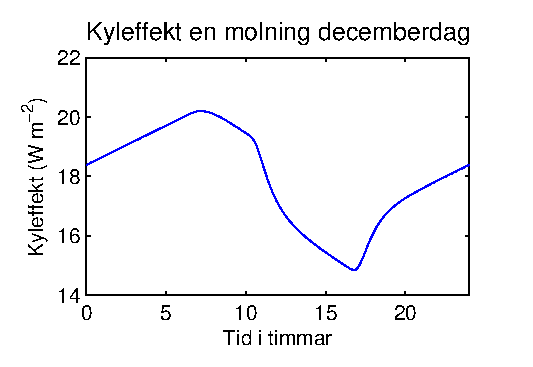
\includegraphics[width=6cm]{images/baynosundec.eps}
}
\caption{\label{fig:bursprak_energi}Energiflödet genom burspråket.}
\end{figure}

Genom burspråket ser energiflödet lite annorlunda ut, figur \ref{fig:bursprak_energi}. En aprilmorgon, innan solen har gått upp, maximeras energiutflödet 10 $\unit{W m^{-2}}$. När solen sedan värmer väggen börjar energi istället flöda in i byggnaden och en riktigt solig dag är det maximala inflödet nästan 20 $\unit{W m^{-2}}$, se figur \ref{fig:bursprak_april1}. En molnig dag stannar det istället på ungefär 1 $\unit{W m^{-2}}$ ut ur väggen, se figur \ref{fig:bursprak_april2}

 En molnig dag  i december är det betydligt kallare och energiutflödet varierar mellan 15 och 20 $\unit{W m^{-2}}$, se figur \ref{fig:bursprak_dec}. En intressant detalj är att kyleffekten på burspråket inte alls är sinusformad, så som flödet genom väggarna i figur \ref{fig:energyflow_stst} och \ref{fig:wall_dec}. Det beror troligen på att väggen är väldigt tunn och reagerar snabbt på olika förändringar.

%%%%%%%%%%%%%%%%%%%%%%%%%%%%%%%%%%%%%%%%%%%%
\paragraph{Temperaturfördelningen utanför väggen}

Även temperaturfödelningen utanför en vägg har beräknats, vilket kan ses i figur \ref{fig:temp_dist}. Det gjordes med finita element metoden applicerad på penaltymetoden.

Temperaturen inne har satts till $\unit[20]{^\circ C}$ och referenstemperaturen ute till 
$\unit[0]{^\circ C}$. Vid fri luft är det ett konvektionsvillkor med konvektionskoefficient 
som motsvarar stillastående luft. Energin som kommer ut från väggen motsvarar 
$U = \unit[1,18]{Wm^{-2}K^{-1}}$. Som kan ses så existerar anomala temperaturer längs 
nedre kanten vilket möjligen kan bero på valet av baselement. Ett bättre val skulle möjligtvis vara metoden Streamline-Upwind/Petrov-Galerkin (SUPG).

%SUPG är en metod, inte flera

\begin{figure}[hpbt]
\centering
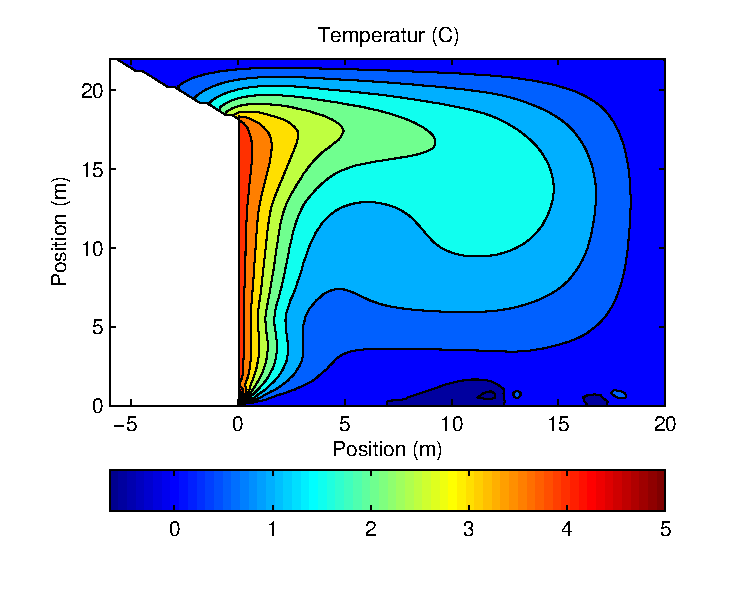
\includegraphics[width=10cm]{images/convectemperature.eps}
\caption{\label{fig:temp_dist}Temperaturfördelningen i $^\circ\mbox{C}$ utanför en vägg, beräknad med finita element av penaltymetoden. Inomhustempertur $\unit[20]{^\circ C}$, utomhustemperatur $\unit[0]{^\circ C}$.}
\end{figure}

% RESULTAT
Som kan ses i figuren \ref{fig:temp_dist} är luften närmast väggen upp till fem grader 
högre än omgivningen. När det blåser försvinner den här temperaturskillnaden. Detta 
visar tydligt hur viktigt det är att inte bara reglera efter utomhustemperaturen. 

%%%%%%%%%%%%%%%%%%%%%%%%%%%%%%%%%%%%%%%%%%%%

Även hastighetsfältet för temperaturens flöde, då det är vindstilla, har beräknats med finita element metoden 
applicerad på penaltymetoden. Detta kan ses i figur \ref{fig:velocityfield} där också 
beloppet av hastighetsfältet syns och det kan noteras att hastigheterna orimligt små.

\begin{figure}[hpbt]
\begin{center}
\subfloat[Hastighetsfält]{
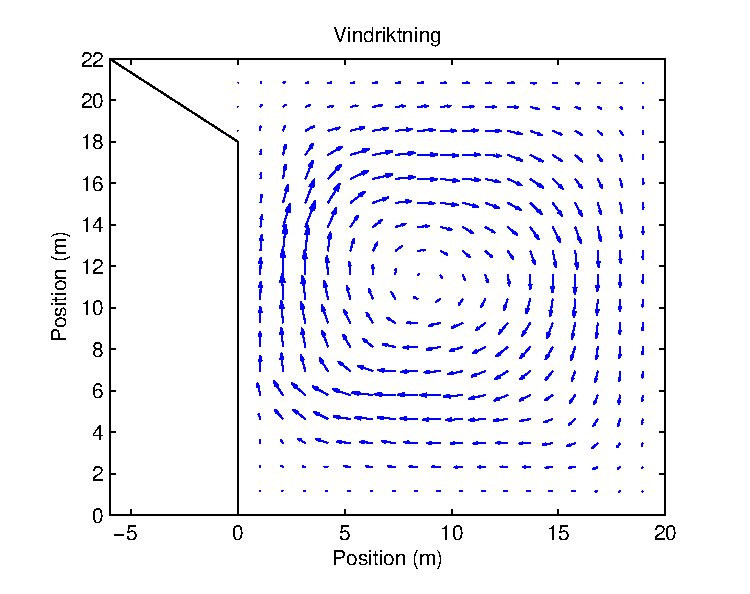
\includegraphics[scale=0.5]{images/convecquiver.eps}
}
\subfloat[Beloppet av hastigheten]{
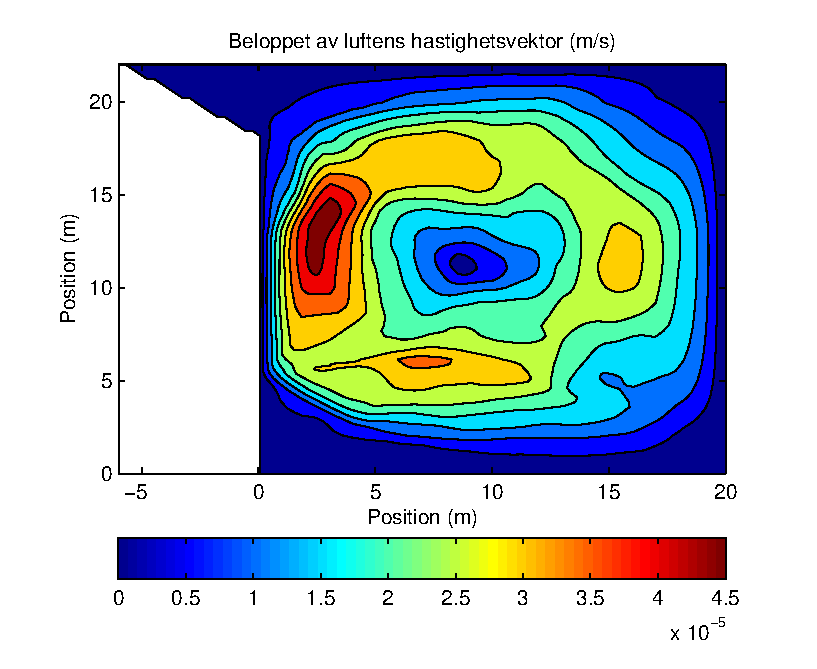
\includegraphics[scale=0.5]{images/convecspeed.eps}
}
\caption{\label{fig:velocityfield} Hur luften vid husväggen flödar vid en temperaturskillnad.}
\end{center}
\end{figure}

Då vi i sedan utifrån detta beräknar konvektionsparametern blir den därför väldigt liten, 
se figur \ref{fig:konv_param}. Tyvärr verkade det inte som att metodiken som användes 
för att framställa ovanstående data fungerade tillräckligt bra för att med någon 
noggrannhet studera fenomenet konvektion.  Vi menar dock att formen på hastighetsflödet intill marken och väggen
kan anses vara av rätt karaktär och visar på hur luften rör sig vid husväggen. Dock kan randerna mot
luft påverka då det ej var tillåtet för luften att passera de
kanterna. Detta kan också vara en felkälla till den absurt låga konvektionsparametern.


\begin{figure}[hpbt]
\centering
\subfloat[\label{fig:h_reftemp}Konvektionskoefficienten h mot referenstemperaturen]{
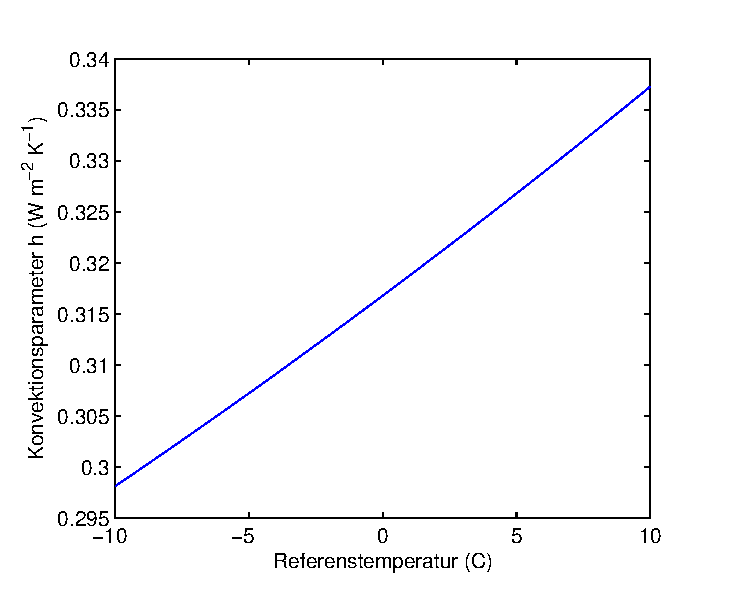
\includegraphics[scale=0.5]{images/convech.eps}
}
\subfloat[\label{fig:h_penalty}Konvektionskoefficienten h mot penaltyparametern]{
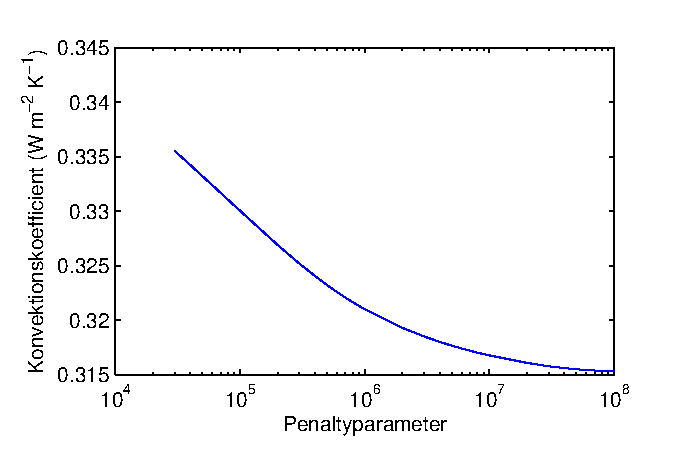
\includegraphics[scale=0.5]{images/convecpenalty.eps}
}\vspace{1cm}

\subfloat[\label{fig:h_volexp}Konvektionskoefficienten h mot den volymetriska expansionskoefficienten.]{
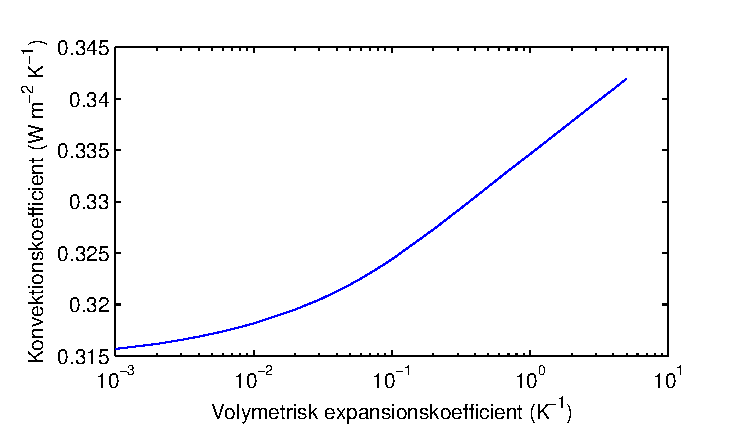
\includegraphics[scale=0.5]{images/convecbeta.eps}
}

\caption{\label{fig:konv_param}Stabilitetsberäkningar av konvektionskoefficienten h mot några
parametrar och naturkonstanter i finita elementsimuleringen av Navier-Stokes ekvationer.
Inomhustemperaturen är satt till konstanta $\unit[20]{^\circ C}$ med en vägg vars U-värde är
$\unit[1,18]{ Wm^{-2}K^{-1}}$. Detta skall motsvara söderväggen på fastigheten som detta arbete behandlar.}

\end{figure}

% RESULTAT
I figur \ref{fig:h_reftemp} har finita elementmodellens beteende studerats vid variation på några essentiella storheter i modellen.
Först har penaltyparametern varierats i figur \ref{fig:h_penalty} och här kan det ses att modellens beteende förändras inte nämnvärt
beroende på val av parameter när denna börjar vara i storleksordningen $\lambda = 10^7$. Det linjära förhållandet mellan
konvektionskoefficienten och temperaturdifferansen är intressant men saknar stöd i litteraturen då den rimligtvis borde vara
konstant eller nästan konstant. Slutligen varieras den volymetriska expansionskoefficienten
i figur \ref{fig:h_volexp}. Det är denna storhet
som gör att luften stiger när den blir varm och av denna anledning fenomenet fri konvektion uppstår. Konvektionskoefficienten
ser ut att öka mer än logaritmiskt men däremot ej så snabbt. Anledningen till att denna parameter varierades var för
att se hur stor den parametern skulle behöva bli innan konvektionen började få samma energitransporterande egenskaper
som den borde ha. Som kan ses så kommer inte modellen ens i närheten vid en väldigt stort vald volymetrisk expansionskoefficient.



\subsection{Flöde genom en vägg vid transient förlopp}

%To regerenate the figures use /code/pdesolver/calculateRisetime.m
%with the argument /code/pdesolver/wallstep.mat

För att visualisera hur flödet genom en vägg förändras med
förändringar i vädret utomhus modelleras ett tidssteg där utomhustemperaturen förändras från 0 till $\unit[10]{^\circ C}$. Inomhustemperaturen hålls konstant till $\unit[20]{^\circ C}$. Detta har gjorts för en vägg utan och en vägg med isolering, se figur \ref{fig:energyflow_trans}. Beräkningarna är genomförda med finita elementmetoden där den oisolerade väggen består av $\unit[0,5]{m}$ tegel och den isolerade har dessutom $\unit[0,1]{m}$ mineralull.

Falltiden för dessa två väggar beräknades till $\unit[34,8]{timmar}$ för väggen utan isolering respektive $\unit[98,8]{timmar}$ för väggen med isolering. 
Värt att notera är också att det tog $\unit[9,6]{timmar}$ respektive $\unit[16,8]{timmar}$ för energiflödet att falla $\unit[10]{\%}$. 

\begin{figure}[hpbt]
\centering

\subfloat[Energiflöde ut från insidan av en oisolerad vägg.]{
\includegraphics[width=6cm]{images/noinsulationstep.eps}
}\vspace{5mm}
\subfloat[Energiflöde ut från insidan av en isolerad vägg]{
\includegraphics[width=6cm]{images/insulationstep.eps}
}
\caption{\label{fig:energyflow_trans} Energiflödet ut från insidan av en vägg. Vid tiden $t<0$ råder jämviktsläge med $\unit[0]{^\circ C}$ på utsidan och $\unit[20]{^\circ C}$ inomhus. Utomhustemperaturen förändras vid tiden $t=0$ i ett steg till $\unit[10]{^\circ C}$. De streckade linjerna markerar $\unit[10]{\%}$ stigning och $\unit[90]{\%}$ stigning.}

\end{figure}

Här kan alltså ses en avsevärd skillnad i hur lång tid det tar innan väggen har anpassat sig till en ny temperatur. En sådan här plötslig och drastisk förändring i temperaturen är inte något som sker speciellt ofta och ju kortare dagarna är destå mindre är temperaturvariationerna mellan dag och natt. \cite{SMHItempskillnad}
Vid nyår kan man inte förvänt sig en skilland på mer än $\unit[2-3]{^\circ C}$. Vi kan ändå konstatera att förändringen i temperatur fortplantar sig betydligt långsammare i en isolerad vägg än en oisolerad. Har man då väggar som är olika bra isolerade behöver man troligen även ha två olika reglersystem för de delar av huset som ligger närmast respektive vägg, om man inte reglerar enbart efter inomhustemperaturen. 

Återigen visas det att en isolerad vägg är mer motståndskraftig för förändringar i utomhustemperaturen vilket är en fördel om ett jämt inomhusklimat eftersträvas.


\subsubsection{Luftfuktighetens inverkan på energiflöden}

\subsection{Luftflöde genom väggar – drag}
\label{sec:leakagewall}

När det blåser på fastigheten får det luften kring fastigheten att cirkulera och även tränga in i 
byggnaden. När vinden ligger på med $\unit[3]{m~s^{-1}}$, vinkelrätt mot nord- eller sydfasaden fås 
ett flöde som det i figur~\ref{fig:windspeed} och trycket som då uppstår visas i figur~
\ref{fig:windpressure}. Tryckskillnaderna på de olika sidorna av husen kommer att driva 
ofrivillig ventilation vilket leder till energiförluster i form av infiltration.

\begin{figure}[hpbt]
\centering
\includegraphics[width=127mm,height=76mm]{images/wind3mshdpi.eps}
\caption{\label{fig:windspeed}Vindhastiheten när vind i $\unit[3]{m~s^{-1}}$ blåser mot fastigheten 
från vänster sida i figuren. Linjerna är strömlinjer och färgen indikerar farten. Värdena är 
framräknade med \emph{Comsol Multiphysics}. Enhet $\unit{m~s^{-1}}$.}
\end{figure}


\begin{figure}[hpbt]
\centering
\includegraphics[width=127mm,height=76mm]{images/pressure3mshdpi.eps}

\caption{\label{fig:windpressure}Lufttrycket när vind i $\unit[3]{m~s^{-1}}$ blåser mot fastigheten från vänster sida i figuren. Linjerna är isobarer, färgen indikerar lufttryck. Värdena är framräknade med
\emph{Comsol Multiphysics}. Enhet Pa.}
\end{figure}

% Resultat
Ur figur~\ref{fig:windspeed} fås att det hus som ligger i lä inte utsätts för någon vind att tala om.
 Vidare fås ur figur~\ref{fig:windpressure} att huset i lä utsätts för en betydligt mindre 
 tryckskillnad, än den byggnad som det blåser direkt på. I vårt exempel här, med en 
 vindhastighet omring $\unit[3]{m~s^{-1}}$ fås en maximal tryckskillnad mellan norr- och sydväggarna.
 på 40 Pa, för fastigheten i lovart. Tryckskillnaden ökar med stigande vindhastighet och vid $\unit[10]{m~s^{-1}}$ fås en 
 tryckskillnad på $\unit[340]{Pa}$ för fastigheten i lovart. 

Applicerat på fastigheten på Walleriusgatan betyder detta att sydvindar ger upphov till 
betydligt mer infiltrationsförluster än nordvindar. Till den aktuella byggnadens fördel ska nämnas 
att södervindarna ofta är varmare än nordvindarna och de faktiska energiförlusterna 
troligen blir något mindre.

%%%%%%%%%%%%%%%%%%%%%%%%%%%%%%%%%%%%%%%%

Energiförlusterna på grund av drag har beräknats utifrån att en bestämd mängd energi per grad finns lagrad i en viss volym luft. Luftflödet genom väggen har beräknats på flera sätt, både med Darcys lag och med byggfysikformeln, se avsnitt~\ref{subsec:darcy}.

Energiförlusten har beräknats
  för en fastighet i lovart respektive en som ligger i lä av en annan byggnad, precis som 
  byggnaderna i figur~\ref{fig:windspeed} och \ref{fig:windpressure}, vilket motsvarar att det 
  blåser på fastigheten på Walleriusgatan från söder respektive norr. Resultatet kan ses i figur~
  \ref{fig:windenergyloss} för en byggnad i lovart och en i lä samt för ett teoretiskt framtaget hus. Dessa två olika kurvor, framtagna med Darcys lag samt med byggfysikformeln, får motsvara högsta respektive minsta gissningar för infiltrationsförluster i en byggnad. \emph{\color{red} Vad representerar den teoretiska huset? Vad vill vi säga med det?}

Trycken i figur~\ref{fig:windenergylossa} och \ref{fig:windenergylossb} är framräknade för 
olika vindhastigheter med programmet \emph{Comsol Multiphysics} medan den teoretiska modellen i figur~
\ref{fig:windenergylossc} är beräknad med med en approximation. 

Approximationen\emph{\color{red} Vilken approximation} baserar sig på att tryckskillnaden mellan inne och ute är proportionerligt mot vindhastigheten i kvadrat. Denna visar hur kyleffekten blir på en fristående rätblocksformad byggnad. Den exakta kyleffekten beror till stor del på vilken omgivning byggnaden står i. \emph{\color{red} Denna förklaring på teoretiska huset är tunn och förvirrad.}


\begin{figure}[hpbt]
\centering
\subfloat[\label{fig:windenergylossa}Byggnad som vinden blåser direkt på.]{
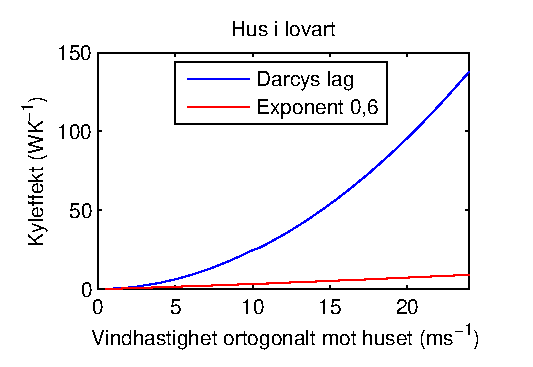
\includegraphics[width=60mm]{images/pressurewind.eps}}
\vspace{5mm}
\subfloat[\label{fig:windenergylossb}Byggnad som ligger i lä av en annan byggnad.]{
\includegraphics[width=60mm]{images/pressurenowind.eps}}

\subfloat[\label{fig:windenergylossc}Teoretisk approximation för lådformad byggnad.]{
\includegraphics[width=60mm]{images/pressuretheory.eps}}

\caption{\label{fig:windenergyloss}Energiförlust per grad, max- respektive minvärde.
Framtaget med \emph{Comsol Multiphysics} (a och b) och teoretiskt framräknade med en approximation (c).}
\end{figure}

% Resultat
Vilken kyleffekt vinden har på fastigheten är mer osäkert vid högre vindhastigheter. När vinden
 ligger på med uppemot $\unit[25]{m~s^{-1}}$ kan kyleffekten variera från några tiotal $\unit{W~m^{-2}~K^{-1}}$ upp 
 emot drygt 100. Motsvarande kan kyleffekt för ett hus i lä vara mellan några $\unit{W~m^{-2}~K^{-1}}$ upp mot knappt 30. För det teoretiskt beräknade huset fås även där att kyleffekten 
 kan vara mellan några $\unit{W~m^{-2}~K^{-1}}$ upp mot knappt 30 $\unit{W~m^{-2}~K^{-1}}$. När vi har mer normala $\unit[10]{m~s^{-1}}$ ser vi istället att kyleffekten kan vara från några få upp emot $\unit[20]{W~m^{-2}~K^{-1}}$ för en byggnad i 
 lovart, och ungefär en fjärdedel av det för en byggnad i lä.
 
För fastighetens norrvägg, den som ligger i lä av en annan fastighet, fås infiltrationsförluster upp till $\unit[28]{kW}$ vid $\unit[10]{m~s^{-1}}$ och temperaturen $\unit[5]{^\circ C}$, då den har arean $\unit[379]{m^2}$. För söderväggen, som ligger mer fritt och har arean $\unit[307]{m^2}$ fås förluster upp till $\unit[115]{kW}$ vid samma vindhastighet. Detta är med beräkningar ur Darcys lag vilket kan anses vara extremt högt räknat och det är mycket otroligt att huset läcker så mycket.




\subsubsection{Solstrålning genom fönster}

Exempel på resultat från beräkningar på solstrålning genom fönster. Beräknat via trial.m i code-mappen.

I figur \ref{fig:vinklar120401} ses de relevanta vinklar som bildas av solens position den första april, 2012. Den blå linjen i figuren representerar solens vinkel relativt ett fönsters normal (då denna pekar i horisontell sydlig riktning) och kan användas för att uppskatta effekten som solinstrålning bidrar till. Om solens intensitet antas vara konstant $\unit{200}{W/m^2}$ beräknas denna effekt motsvara vad som visas i figur \ref{fig:effekt120401}. Här antas fönstrets area uppgå till $\unit{1.5}{m^2}$, g-värdet för normal solstrålning är ? och värdet p i koden sätts till ?, ty fönstren i den avsedda byggnaden är av typ treglas utan ytbeläggningar.

\begin{figure}[hpbt]
\centering
\includegraphics[scale=1]{images/angles120401.eps}
\caption{\label{fig:vinklar120401} Beräknade vinklar vid Walleriusgatan den första april 2012, tid i UTC}
\end{figure}

\begin{figure}[hpbt]
\centering
\includegraphics[scale=1]{images/effekt120401.eps}
\caption{\label{fig:effekt120401} Beräknad effekt genom ett fönster vars normal pekar i horisontella sydriktningen, den första april 2012. Solens intensitet tas konstant till 200 W/m$^2$}
\end{figure}


\section{Energiflöde genom grunden}

\subsubsection{Flöde vid termisk jämvikt}

Vid beräkningen av värmeflödet genom grunden användes geometrin som kan ses i figur \ref{fig:groundheat}.
Källaren antas vara belägen en halv meter under marknivån.

Som kan ses så varierar ej energiflödet så mycket mellan årstiderna och antags därför vara konstant i många applikationer.


\emph{\color{red} Nedanstående text måste göras om med de nya figurerna i åtanke,}
I samma figur ses även temperaturfördelningen vid termisk jämvikt då markens temperatur långt under huset sätts till konstanta $\unit[8]{^{circ}C}$. Vid markytan sattes konvektionskoefficienten till $h=\unit[15,5]{Wm^{-2}K^{-1}}$, motsvarande en ungefärlig vindhastighet (parallel med ytan) på $\unit[2]{ms^{-1}}$ vid utomhustemperaturen $\unit[0]{^{\circ}C}$. Källarens temperatur antas vara konstant $\unit[10]{^{\circ}C}$ och \textcolor{red}{grundens U-värde approximeras till $\unit[?]{Wm^{-2}K^{-1}}$}.


\begin{figure}
\centering
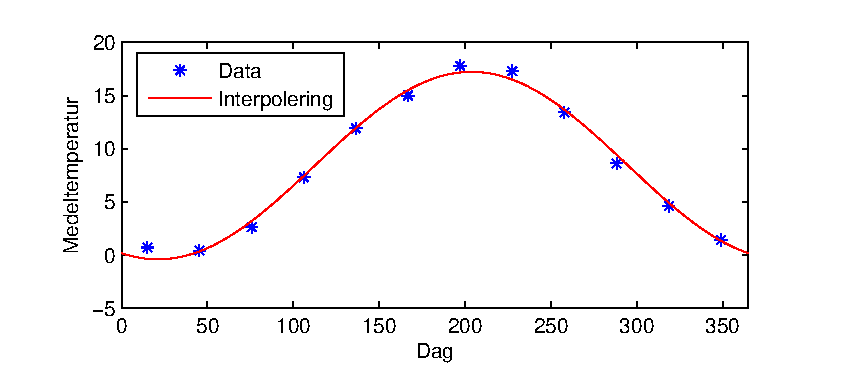
\includegraphics{images/meantemperature.eps}
\caption{Medeltemperaturen för göteborg de senaste 20 åren. Punkterna är data tagna från Miljöförvaltningen
och linjen är minstakvadratanpassningen som senare använts för att beräkna energiflöden.
\emph{\color{red} Denna graf kanske inte ska ligga här eller alls vara med. Metod möjligtvis? Vad tycker ni?}}
\end{figure}

\begin{figure}
\centering
\subfloat[Temperaturfördelningen i $^\circ\mbox{C}$ första januari.]{
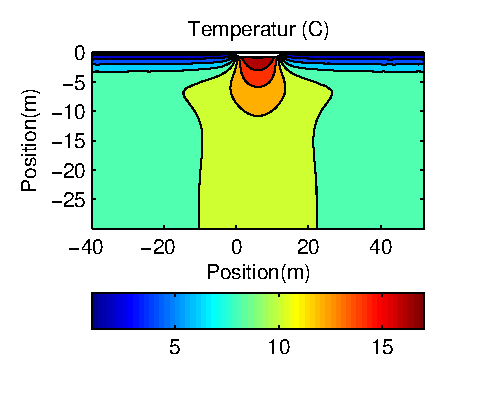
\includegraphics{images/groundheatdec.eps}
}

\subfloat[Temperaturfördelningen i $^\circ\mbox{C}$ första juli.]{
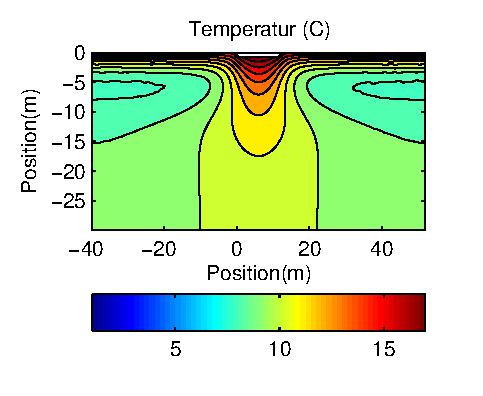
\includegraphics{images/groundheatjune.eps}
}
\caption{\label{fig:groundheat}Temperaturen i marken under en byggnad angivet i grader Celsius.
Temperaturfördelningarna skall motsvara två fiktiva dagar under ett år som är baserad på månadsmedeltemperaturen
de senaste 20 åren i Göteborg. Konvektionsparametern är satt till $h=15,5$. }
\end{figure}


\begin{figure}
\centering
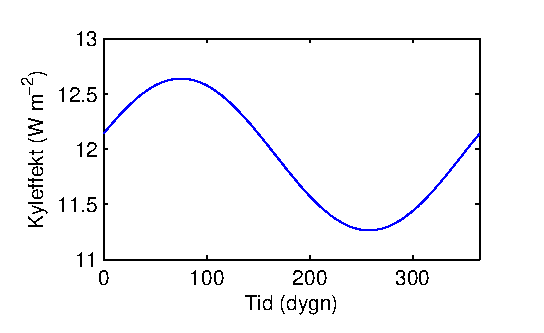
\includegraphics{images/groundcool.eps}
\caption{Kyleffekten per $m^2$ från grunden för medelåret de senaste tjugo åren. \emph{\color{red} Samma parametrar som figuren ovan.}\emph{\color{red}                                     
Detta är en viktig figur. Här kan ses att $\Delta Q = 1.5*22*13 = \unit[439]{W}$. Detta offsettas lätt genom att fler
människor befinner sig i fastigheten på vintern ty det är kallt ute eller fler kollar på tv istället för att sola.
Således finns det inget behov för att reglera framlednigstemperaturen för energiförluster från grunden. Kan antagas konstant
$\approx \unit[3,5]{kW}$. Låter denna siffra rimlig?}}

\end{figure}



\subsection{Flöde vid transient förlopp}


\section{Tidskonstanter}

% Eliminerat avsnitt, kan tas bort

\section{Sammanfattning av energiflöden: free-running temperature}


